\section*{7.4 Estimadores de Bayes}
Um estimador de um parâmetro é alguma função dos dados que esperamos que seja próxima ao parâmetro. Um estimador de Bayes é um estimador que é escolhido para minimizar a média a posteriori de alguma medida de quão longe um estimador está do parâmetro, como o erro quadrático ou o erro absoluto.

\subsection*{Natureza de um Problema de Estimação}

\noindent\textbf{Exemplo 7.4.1} \quad \textbf{Contagem de Calorias em Rótulos de Alimentos.} No Exemplo 7.3.10, encontramos a distribuição a posteriori de $\theta$, a diferença percentual média entre as calorias medidas e as anunciadas. Um grupo de consumidores pode desejar relatar um único número como uma estimativa de $\theta$ sem especificar a distribuição inteira para $\theta$. Como escolher tal estimativa de número único é o assunto desta seção.

Começamos com uma definição apropriada para um valor de variável real, como no Exemplo 7.4.1. Uma definição mais geral se seguirá depois que nos familiarizarmos mais com o conceito de estimação.

\vspace{1cm}
\noindent\textbf{Definição 7.4.1} \quad \textbf{Estimador/Estimativa.} Seja $X_1, \dots, X_n$ observáveis, cuja distribuição conjunta é indexada por um parâmetro $\theta$ assumindo valores em um subconjunto $\Omega$ da reta real. Um \textit{estimador} do parâmetro $\theta$ é uma função de valor real $\delta(X_1, \dots, X_n)$. Se $X_1=x_1, \dots, X_n=x_n$ são observados, então $\delta(x_1, \dots, x_n)$ é chamada de \textit{estimativa} de $\theta$.

\vspace{1cm}
Note que todo estimador é, por natureza de ser uma função dos dados, uma estatística no sentido da Definição 7.1.4.
Como o valor de $\theta$ deve pertencer a $\Omega$, pode parecer razoável exigir que todo valor possível de um estimador $\delta(X_1, \dots, X_n)$ também deva pertencer a $\Omega$. Não exigiremos essa restrição, no entanto. Se um estimador pode assumir valores fora do espaço de parâmetros $\Omega$, o experimentador precisará decidir no problema específico se isso parece apropriado ou se tem propriedades menos desejáveis.
Na Definição 7.1.4, distinguimos entre os termos \textit{estatística} e \textit{estimativa}. Como um estimador $\delta(X_1, \dots, X_n)$ é uma função dos dados, o próprio estimador é uma variável aleatória, e sua distribuição de probabilidade pode ser derivada da distribuição conjunta de $X_1, \dots, X_n$ se esta for conhecida. Por outro lado, uma \textit{estimativa} é o valor específico $\delta(x_1, \dots, x_n)$ do estimador que é determinado usando valores observados específicos $x_1, \dots, x_n$. Se usarmos a notação vetorial $\mathbf{X}=(X_1, \dots, X_n)$ e $\mathbf{x}=(x_1, \dots, x_n)$, então um estimador é uma função $\delta(\mathbf{X})$ do vetor aleatório $\mathbf{X}$, e uma estimativa é um valor específico $\delta(\mathbf{x})$. Muitas vezes será conveniente denotar um estimador $\delta(\mathbf{X})$ simplesmente pelo símbolo $\delta$.

\subsection*{Funções de Perda}

\noindent\textbf{Exemplo 7.4.2} \quad \textbf{Contagem de Calorias em Rótulos de Alimentos.} No Exemplo 7.4.1, o grupo de consumidores pode sentir que, quanto mais distante sua estimativa $\delta(\mathbf{x})$ estiver da verdadeira diferença média $\theta$, mais constrangimento e possíveis ações legais eles enfrentarão. Idealmente, eles gostariam de quantificar a magnitude das repercussões negativas como uma função de $\theta$ e da estimativa $\delta(\mathbf{x})$, e então poderiam ter alguma ideia da probabilidade de encontrar vários níveis de transtorno como resultado de sua estimação. O requisito mais fundamental de um bom estimador $\delta$ é que ele produza uma estimativa de $\theta$ que esteja próxima do valor real de $\theta$. Em outras palavras, um bom estimador é aquele para o qual é altamente provável que o erro $\delta(\mathbf{X}) - \theta$ esteja próximo de 0. Assumiremos que para cada valor possível de $\theta \in \Omega$ e cada estimativa possível $a$, existe um número $L(\theta, a)$ que mede a perda ou o custo para o estatístico quando o verdadeiro valor do parâmetro é $\theta$ e sua estimativa é $a$. Normalmente, quanto maior a distância entre $a$ e $\theta$, maior será o valor de $L(\theta, a)$.

\vspace{1cm}
\noindent\textbf{Definição 7.4.2} \quad \textbf{Função de perda.} Uma \textit{função de perda} é uma função de valor real de duas variáveis, $L(\theta, a)$, onde $\theta \in \Omega$ e $a$ é um número real. A interpretação é que um estatístico perde $L(\theta, a)$ se o parâmetro for igual a $\theta$ e a estimativa for igual a $a$.

\vspace{1cm}
Como antes, seja $\xi(\theta)$ a f.d.p. a priori de $\theta$ no conjunto $\Omega$, e considere um problema no qual o estatístico deve estimar o valor de $\theta$ sem poder observar os valores em uma amostra aleatória. Se o estatístico escolher uma estimativa particular $a$, então sua perda esperada será
\begin{equation}
E[L(\theta, a)] = \int_{\Omega} L(\theta, a)\xi(\theta)d\theta. \tag{7.4.1}
\end{equation}
Assumiremos que o estatístico deseja escolher uma estimativa $a$ para a qual a perda esperada em Eq. (7.4.1) é um mínimo.

\subsection*{Definição de um Estimador de Bayes}
Suponha agora que o estatístico possa observar o valor $\mathbf{x}$ do vetor aleatório $\mathbf{X}$ antes de estimar $\theta$, e seja $\xi(\theta|\mathbf{x})$ a f.d.p. a posteriori de $\theta$ no conjunto $\Omega$. (O caso de um parâmetro discreto pode ser tratado de maneira semelhante.) Para cada estimativa $a$ que o estatístico possa usar, sua perda esperada neste caso será
\begin{equation}
E[L(\theta, a)|\mathbf{x}] = \int_{\Omega} L(\theta, a)\xi(\theta|\mathbf{x})d\theta. \tag{7.4.2}
\end{equation}
Portanto, o estatístico deve agora escolher uma estimativa $a$ para a qual a esperança em Eq. (7.4.2) é um mínimo.
Para cada valor possível $\mathbf{x}$ do vetor aleatório $\mathbf{X}$, seja $\delta^*(\mathbf{x})$ o valor de uma estimativa $a$ para a qual a perda esperada em Eq. (7.4.2) é um mínimo. Então o estimador $\delta^*(X)$ para o qual os valores são especificados desta forma será um estimador de $\theta$.

\vspace{1cm}
\noindent\textbf{Definição 7.4.3} \quad \textbf{Estimador/Estimativa de Bayes.} Seja $L(\theta, a)$ uma função de perda. Para cada valor possível $\mathbf{x}$ de $\mathbf{X}$, seja $\delta^*(\mathbf{x})$ um valor de $a$ tal que $E[L(\theta, a)|\mathbf{x}]$ é minimizado. Então $\delta^*$ é chamado de \textit{Estimador de Bayes} de $\theta$. Uma vez que $\mathbf{X}=\mathbf{x}$ é observado, $\delta^*(\mathbf{x})$ é chamado de \textit{Estimativa de Bayes} de $\theta$.

\vspace{1cm}
Outra maneira de descrever uma estimativa de Bayes $\delta^*(\mathbf{x})$ é notar que, para cada valor possível $\mathbf{x}$ de $\mathbf{X}$, o valor $\delta^*(\mathbf{x})$ é escolhido de modo que
\begin{equation}
E[L(\theta, \delta^*(\mathbf{x}))|\mathbf{x}] = \min_{a} E[L(\theta, a)|\mathbf{x}]. \tag{7.4.3}
\end{equation}
Em resumo, consideramos um problema de estimação no qual uma amostra aleatória $\mathbf{X}=(X_1, \dots, X_n)$ deve ser retirada de uma distribuição envolvendo um parâmetro $\theta$ que tem um valor desconhecido em algum conjunto especificado $\Omega$. Para cada função de perda $L(\theta, a)$ e cada f.d.p. a priori $\xi(\theta)$ dadas, o estimador de Bayes de $\theta$ é o estimador $\delta^*(\mathbf{X})$ para o qual a Eq. (7.4.3) é satisfeita para cada valor possível $\mathbf{x}$ de $\mathbf{X}$. Deve ser enfatizado que a forma do estimador de Bayes dependerá tanto da função de perda que é usada no problema quanto da distribuição a priori que é atribuída a $\theta$. Nos problemas descritos neste texto, os estimadores de Bayes existirão. No entanto, existem situações mais complicadas nas quais nenhuma função $\delta^*$ satisfaz (7.4.3).

\subsection*{Diferentes Funções de Perda}
De longe, a função de perda mais comumente usada em problemas de estimação é a função de perda de erro quadrático.

\vspace{1cm}
\noindent\textbf{Definição 7.4.4} \quad \textbf{Função de Perda de Erro Quadrático.} A função de perda
\begin{equation}
L(\theta, a) = (\theta-a)^2 \tag{7.4.4}
\end{equation}
é chamada de \textit{perda de erro quadrático}.

\vspace{1cm}
Quando a função de perda de erro quadrático é usada, a estimativa de Bayes $\delta^*(\mathbf{x})$ para cada valor observado de $\mathbf{x}$ será o valor de $a$ para o qual a esperança $E[(\theta-a)^2|\mathbf{x}]$ é um mínimo. O Teorema 4.7.3 afirma que a esperança de $(\theta-a)^2$ é calculada com respeito a uma certa distribuição de $\theta$, esta esperança será um mínimo quando $a$ for escolhido como igual à média $E(\theta|\mathbf{x})$ da distribuição a posteriori, se a média a posteriori for finita. Se a média a posteriori não for finita, então a perda esperada é infinita para cada valor possível de $a$. Portanto, temos o seguinte corolário do Teorema 4.7.5.

\vspace{1cm}
\noindent\textbf{Corolário 7.4.1} \quad Seja $\theta$ um parâmetro de valor real. Suponha que a função de perda de erro quadrático (7.4.4) seja usada e que a média a posteriori, $E(\theta|\mathbf{X})$, seja finita. Então, um estimador de Bayes de $\theta$ é $\delta^*(\mathbf{X}) = E(\theta|\mathbf{X})$.

\vspace{1cm}
\noindent\textbf{Exemplo 7.4.3} \quad \textbf{Estimando o Parâmetro de uma Distribuição de Bernoulli.} Seja a amostra aleatória $X_1, \dots, X_n$ da distribuição de Bernoulli com parâmetro $\theta$, que é desconhecido e deve ser estimado. Seja a distribuição a priori de $\theta$ a distribuição beta com parâmetros $\alpha>0$ e $\beta>0$. Suponha que a função de perda de erro quadrático seja usada, como especificado em Eq. (7.4.4), para $0<\theta<1$ e $0<a<1$. Determinaremos a estimativa de Bayes de $\theta$.
Para valores observados $x_1, \dots, x_n$, seja $y=\sum_{i=1}^{n}x_i$. Segue-se do Teorema 7.3.1 que a distribuição a posteriori de $\theta$ será a distribuição beta com parâmetros $\alpha_1=\alpha+y$ e $\beta_1=\beta+n-y$. Uma vez que a média da distribuição beta com parâmetros $\alpha_1$ e $\beta_1$ é $\alpha_1/(\alpha_1+\beta_1)$, a média da distribuição a posteriori de $\theta$ será $(\alpha+y)/(\alpha+\beta+n)$. A estimativa de Bayes $\delta^*(\mathbf{x})$ será igual a este valor para cada vetor observado $\mathbf{x}$. Portanto, o estimador de Bayes $\delta^*(\mathbf{X})$ é especificado da seguinte forma:
\begin{equation}
\delta^*(\mathbf{X}) = \frac{\alpha+\sum_{i=1}^{n}X_i}{\alpha+\beta+n}. \tag{7.4.5}
\end{equation}

\noindent\textbf{Exemplo 7.4.4} \quad \textbf{Estimando a Média de uma Distribuição Normal.} Seja a amostra aleatória $X_1, \dots, X_n$ de uma distribuição normal para a qual o valor da média $\theta$ é desconhecido e o valor da variância $\sigma^2$ é conhecido. Suponha também que a distribuição a priori de $\theta$ seja uma distribuição normal com média $\mu_0$ e variância $\nu_0^2$. Finalmente, suponha que a função de perda de erro quadrático seja usada, como especificado em Eq. (7.4.4), para $-\infty<\theta<\infty$ e $-\infty<a<\infty$. Determinaremos o estimador de Bayes de $\theta$.
Segue-se do Teorema 7.3.3 que para todos os valores observados $x_1, \dots, x_n$, a distribuição a posteriori de $\theta$ será a distribuição normal com média $\mu_1$ especificada em Eq. (7.3.1). Portanto, o estimador de Bayes $\delta^*(\mathbf{X})$ é especificado da seguinte forma:
\begin{equation}
\delta^*(\mathbf{X}) = \frac{\sigma^2\mu_0+n\nu_0^2\bar{X}_n}{\sigma^2+n\nu_0^2}. \tag{7.4.6}
\end{equation}
A variância a posteriori de $\theta$ não entra neste cálculo.

Outra função de perda comumente usada em problemas de estimação é a função de perda de erro absoluto.

\vspace{1cm}
\noindent\textbf{Definição 7.4.5} \quad \textbf{Função de Perda de Erro Absoluto.} A função de perda
\begin{equation}
L(\theta, a) = |\theta-a| \tag{7.4.7}
\end{equation}
é chamada de \textit{perda de erro absoluto}.

\vspace{1cm}
Para cada valor observado de $\mathbf{x}$, a estimativa de Bayes $\delta^*(\mathbf{x})$ será agora o valor de $a$ para o qual a esperança $E(|\theta-a||\mathbf{x})$ é um mínimo. Foi mostrado no Teorema 4.5.3 que para cada distribuição de probabilidade dada de $\theta$, a esperança de $|\theta-a|$ será um mínimo quando $a$ for escolhido como a mediana da distribuição de $\theta$. Portanto, quando a esperança de $|\theta-a|$ é calculada com respeito à distribuição a posteriori de $\theta$, esta esperança será um mínimo quando $a$ for escolhido como a mediana da distribuição a posteriori de $\theta$.

\vspace{1cm}
\noindent\textbf{Corolário 7.4.2} \quad Quando a função de perda de erro absoluto (7.4.7) é usada, um estimador de Bayes de um parâmetro de valor real $\theta$ é $\delta^*(\mathbf{X})$ igual a uma mediana da distribuição a posteriori de $\theta$.

\vspace{1cm}
Vamos agora reconsiderar os Exemplos 7.4.3 e 7.4.4, mas usaremos a função de perda de erro absoluto em vez da função de perda de erro quadrático.

\vspace{1cm}
\noindent\textbf{Exemplo 7.4.5} \quad \textbf{Estimando o Parâmetro de uma Distribuição de Bernoulli.} Considere novamente as condições do Exemplo 7.4.3, mas suponha que a função de perda de erro absoluto seja usada, como especificado na Eq. (7.4.7). Para todos os valores observados $x_1, \dots, x_n$, a estimativa de Bayes $\delta^*(\mathbf{x})$ será igual à mediana da distribuição a posteriori de $\theta$, que é a distribuição beta com parâmetros $\alpha+y$ e $\beta+n-y$. Não há expressão simples para a mediana desta distribuição. Ela deve ser determinada por aproximações numéricas para cada conjunto de valores observados. A maioria dos softwares de computador estatísticos pode calcular a mediana de uma distribuição beta arbitrária.
Como um exemplo específico, considere a situação descrita no Exemplo 7.3.13 no qual uma priori imprópria foi usada. A distribuição a posteriori de $\theta$ nesse exemplo foi a distribuição beta com parâmetros 22 e 18. A média desta distribuição beta é $22/40 = 0.55$. A mediana é 0.5508.

\vspace{1cm}
\noindent\textbf{Exemplo 7.4.6} \quad \textbf{Estimando a Média de uma Distribuição Normal.} Considere novamente as condições do Exemplo 7.4.4, mas suponha agora que a função de perda de erro absoluto seja usada, como especificado na Eq. (7.4.7). Para todos os valores observados, a estimativa de Bayes $\delta^*(\mathbf{x})$ será igual à mediana da distribuição normal a posteriori de $\theta$. No entanto, uma vez que a média e a mediana de cada distribuição normal são iguais, $\delta^*(\mathbf{x})$ é igual à média da distribuição a posteriori. Portanto, o estimador de Bayes com respeito à função de perda de erro absoluto é o mesmo que o estimador de Bayes com respeito à função de perda de erro quadrático, e é novamente dado pela Eq. (7.4.6).

\subsection*{Outras Funções de Perda}
Embora a função de perda de erro quadrático e, em menor grau, a função de perda de erro absoluto sejam as funções de perda mais comumente usadas em problemas de estimação, nenhuma delas pode ser apropriada em um problema de estimação particular. Em alguns problemas, pode ser apropriado usar uma função de perda com a forma $L(\theta, a)=|\theta-a|^k$, onde $k$ é algum número positivo diferente de 1 ou 2. Em outros problemas, o fato de a estimativa $a$ ter uma magnitude grande pode depender do valor real de $\theta$. Em tal problema, pode ser apropriado usar uma função de perda com a forma $L(\theta, a) = \lambda_1(\theta)|\theta-a|$ ou $L(\theta, a)=\lambda_2(\theta)(\theta-a)^2$, onde $\lambda(\theta)$ é uma função positiva de $\theta$. Em outros problemas ainda, pode ser mais custoso superestimar $\theta$ por uma certa quantidade do que subestimá-lo pela mesma quantidade. Uma função de perda específica que reflete essa propriedade é a seguinte:
$$ L(\theta, a) =
\begin{cases}
3(\theta-a)^2 & \text{para } \theta \le a, \\
(\theta-a)^2 & \text{para } \theta > a.
\end{cases}
$$
Vários outros tipos de funções de perda podem ser relevantes em problemas de estimação específicos. No entanto, neste livro, daremos a maior parte de nossa atenção às funções de perda de erro quadrático e de erro absoluto.

\subsection*{A Estimativa de Bayes para Amostras Grandes}
\noindent\textbf{Efeito de Diferentes Distribuições a Priori.} Suponha que a proporção $\theta$ de itens defeituosos em um grande lote seja desconhecida e que a distribuição a priori de $\theta$ seja a distribuição uniforme no intervalo $[0, 1]$. Suponha também que o valor de $\theta$ deva ser estimado, e que a função de perda de erro quadrático seja usada. Suponha, finalmente, que em uma amostra aleatória de 100 itens do lote, 10 itens sejam defeituosos. Como a distribuição uniforme é a distribuição beta com parâmetros $\alpha=1$ e $\beta=1$, e como $n=100$ e $y=10$, segue-se de Eq. (7.4.5) que a estimativa de Bayes é $\delta^*(\mathbf{x}) = 11/102 = 0.108$.
Agora, suponha que a f.d.p. a priori de $\theta$ tenha a forma $\xi(\theta) = 2(1-\theta)$ para $0<\theta<1$. Em vez de uma distribuição uniforme, e que em uma amostra aleatória de 100 itens, exatamente 10 itens sejam defeituosos. Como $\xi(\theta)$ é a f.d.p. da distribuição beta com parâmetros $\alpha=1$ e $\beta=2$, segue-se de Eq. (7.4.5) que neste caso a estimativa de Bayes de $\theta$ é $\delta(\mathbf{x})=11/103=0.107$.
As duas distribuições a priori consideradas aqui são bastante diferentes. A média da distribuição uniforme é 1/2, e a média da outra distribuição a priori é 1/3. No entanto, como o número de observações na amostra é grande ($n=100$), as estimativas de Bayes com respeito às duas distribuições a priori diferentes são quase as mesmas. Além disso, os valores de ambas as estimativas são muito próximos da proporção observada de itens defeituosos na amostra, $\bar{x}_n = 0.1$.

\vspace{1cm}
\noindent\textbf{Exemplo 7.4.7} \quad \textbf{Medidas de Peito.} Quetelet (1846) relatou (com alguns erros) dados sobre as medidas de peito (em polegadas) de 5732 milicianos escoceses. Esses dados apareceram anteriormente em um artigo de 1817 de um médico militar e foram discutidos por Stigler (1986). A Fig. 7.6 mostra um histograma dos dados. Suponha que modelamos as medidas individuais do peito como uma amostra aleatória (dado $\theta$) de variáveis aleatórias normais com média $\theta$ e variância 4. A média do peito da amostra é $\bar{x}_n = 39.85$. Se tivéssemos a distribuição normal a priori com média $\mu_0$ e variância $\nu_0^2$, então usando a Eq. (7.3.1) a distribuição a posteriori de $\theta$ seria normal com média
$$ \mu_1 = \frac{4\mu_0+5732 \times \nu_0^2 \times 39.85}{4+5732 \times \nu_0^2} $$
e variância
$$ \nu_1^2 = \frac{4\nu_0^2}{4+5732 \times \nu_0^2}. $$
A estimativa de Bayes será então $\delta(\mathbf{x})=\mu_1$. Note que, a menos que $\mu_0$ seja incrivelmente grande ou $\nu_0^2$ seja muito pequeno, teremos $\mu_1$ quase igual a 39.85 e $\nu_1^2$ quase igual a $4/5732$. De fato, se a f.d.p. a priori de $\theta$ for qualquer função contínua que seja positiva em torno de $\theta=39.85$ e não seja extremamente grande longe de 39.85, então a f.d.p. a posteriori de $\theta$ com uma f.d.p. normal muito próxima com média 39.85 e variância $4/5732$. A média e a mediana da distribuição a posteriori estão próximas de 39.85, independentemente da distribuição a priori.

\vspace{1cm}
% [ESPAÇO PARA FIGURA 7.6]
\begin{figure}[H]

\centering

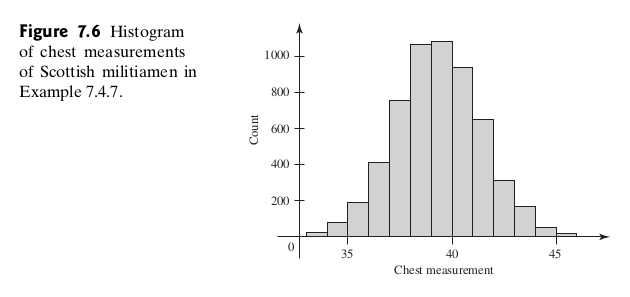
\includegraphics[width=0.5\textwidth]{img/7_4/img_1.png}

\end{figure}
\vspace{1cm}

\noindent\textbf{Consistência do Estimador de Bayes.} Seja $X_1, \dots, X_n$ uma amostra aleatória (dado $\theta$) da distribuição de Bernoulli com parâmetro $\theta$. Suponha que usamos uma priori conjugada para $\theta$. Como $\theta$ é a média da distribuição da qual a amostra está sendo retirada, segue-se das leis dos grandes números discutidas na Seção 6.2 que $\bar{X}_n$ converge em probabilidade para $\theta$ quando $n \to \infty$. Como a diferença entre o estimador de Bayes $\delta^*(\mathbf{X})$ e $\bar{X}_n$ converge em probabilidade para 0 quando $n \to \infty$, também pode ser concluído que $\delta^*(\mathbf{X})$ converge em probabilidade para o valor desconhecido de $\theta$ quando $n \to \infty$.

\vspace{1cm}
\noindent\textbf{Definição 7.4.6} \quad \textbf{Sequência Consistente de Estimadores.} Uma sequência de estimadores que converge em probabilidade para o valor desconhecido do parâmetro que está sendo estimado, quando $n \to \infty$, é chamada de \textit{sequência consistente de estimadores}.

\vspace{1cm}
Assim, mostramos que os estimadores de Bayes $\delta^*(\mathbf{X})$ formam uma sequência consistente de estimadores no problema considerado aqui. A interpretação prática deste resultado é a seguinte: Quando um grande número de observações é feito, há alta probabilidade de que o estimador de Bayes esteja muito próximo do valor desconhecido de $\theta$.
Os resultados que acabamos de apresentar para estimar o parâmetro de uma distribuição de Bernoulli também são verdadeiros para outros problemas de estimação. Sob condições gerais razoáveis e para uma ampla classe de funções de perda, os estimadores de Bayes de alguns parâmetros $\theta$ formarão uma sequência consistente de estimadores à medida que o tamanho da amostra $n \to \infty$. Em particular, para amostras aleatórias de qualquer uma das várias famílias de distribuições discutidas na Seção 7.3, se uma distribuição a priori conjugada for atribuída aos parâmetros e a função de perda de erro quadrático for usada, os estimadores de Bayes formarão sequências consistentes de estimadores.
Por exemplo, considere novamente as condições do Exemplo 7.4.4. Nesse exemplo, uma amostra aleatória é retirada de uma distribuição normal para a qual o valor da média $\theta$ é desconhecido, e o estimador de Bayes $\delta^*(\mathbf{X})$ é especificado por Eq. (7.4.6). Como $\bar{X}_n$ convergirá para o valor desconhecido de $\theta$ quando $n \to \infty$, pode-se ver a partir da Eq. (7.4.6) que $\delta^*(\mathbf{X})$ também convergirá para $\theta$ quando $n \to \infty$. Assim, os estimadores de Bayes novamente formam uma sequência consistente de estimadores. Outros exemplos são dados nos Exercícios 7 e 11 no final desta seção.

\subsection*{Parâmetros e Estimadores Mais Gerais}
Até agora nesta seção, consideramos apenas parâmetros de valor real e estimadores desses parâmetros. Existem duas generalizações muito comuns desta situação que são fáceis de lidar com as mesmas técnicas descritas acima. A primeira generalização é para parâmetros multidimensionais, como o parâmetro bidimensional de uma distribuição normal com média e variância desconhecidas. A segunda generalização é para funções do parâmetro em vez do próprio parâmetro. Por exemplo, se $\theta$ é a taxa de falha no Exemplo 7.1.1, podemos estar interessados em estimar $1/\theta$, o tempo médio até a falha. Como outro exemplo, se nossos dados provêm de uma distribuição normal com média e variância desconhecidas, podemos desejar estimar apenas a média em vez do parâmetro inteiro.
As mudanças necessárias na Definição 7.4.1 para lidar com ambas as generalizações que acabamos de mencionar são dadas na Definição 7.4.7.

\vspace{1cm}
\noindent\textbf{Definição 7.4.7} \quad \textbf{Estimador/Estimativa.} Seja $X_1, \dots, X_n$ observáveis, cuja distribuição conjunta é indexada por um parâmetro $\theta$ assumindo valores em um subconjunto $\Omega$ de um espaço $k$-dimensional. Seja $h$ uma função de $\Omega$ para um espaço $d$-dimensional. Defina $\psi = h(\theta)$. Um \textit{estimador} de $\psi$ é uma função $\delta(X_1, \dots, X_n)$ que assume valores no espaço $d$-dimensional. Se $X_1=x_1, \dots, X_n=x_n$ são observados, então $\delta(x_1, \dots, x_n)$ é chamada de \textit{estimativa} de $\psi$.

\vspace{1cm}
Quando $h$ na Definição 7.4.7 é a função identidade $h(\theta)=\theta$, então $\psi=\theta$ e estamos estimando o parâmetro original $\theta$. Quando $h(\theta)$ é uma coordenada de $\theta$, então $\psi$ é essa coordenada, e estamos estimando apenas essa coordenada.
Haverá uma série de parâmetros multidimensionais em seções posteriores e capítulos deste livro. Aqui está um exemplo de estimar uma função de um parâmetro.

\vspace{1cm}
\noindent\textbf{Exemplo 7.4.8} \quad \textbf{Tempo de Vida de Componentes Eletrônicos.} No Exemplo 7.3.12, suponha que queiramos estimar $\psi=1/\theta$, o tempo médio até a falha dos componentes eletrônicos. A distribuição a posteriori de $\theta$ é a distribuição gama com parâmetros 4 e 8.6. Se usarmos a função de perda de erro quadrático $L(\theta, a)=(\psi-a)^2$, o Teorema 4.7.3 diz que a estimativa de Bayes é a média da distribuição a posteriori de $\psi$. Que é,
\begin{align*}
\delta^*(\mathbf{x}) &= E(\psi|\mathbf{x}) = E\left(\frac{1}{\theta}\bigg|\mathbf{x}\right) \\
&= \int_0^{\infty}\frac{1}{\theta}\xi(\theta|\mathbf{x})d\theta \\
&= \int_0^{\infty}\frac{1}{\theta}\frac{8.6^4}{6}\theta^3 e^{-8.6\theta}d\theta \\
&= \frac{8.6^4}{6}\int_0^{\infty}\theta^2 e^{-8.6\theta}d\theta \\
&= \frac{8.6^4}{6}\frac{2}{8.6^3} = \frac{8.6}{3}=2.867.
\end{align*}
onde a igualdade final segue do Teorema 5.7.3. A média de $1/\theta$ é ligeiramente maior que $1/E(\theta|\mathbf{x}) = 8.6/4 = 2.15$.

\vspace{1cm}
\noindent\textbf{Nota: Funções de Perda e Utilidade.} Na Seção 4.8, introduzimos o conceito de utilidade para medir os valores para um tomador de decisão de vários resultados aleatórios. O conceito de função de perda está intimamente relacionado ao de utilidade. Em um sentido, uma função de perda é como o negativo de uma utilidade. De fato, o Exemplo 4.8.8 mostra como converter perda de erro absoluto em uma utilidade. Nesse exemplo, o papel do parâmetro $\theta$ e do estimador $d(W)$ desempenham os papéis do estimador. De maneira semelhante, pode-se converter outras funções de perda em utilidades. Portanto, não é surpreendente que o objetivo de maximizar a utilidade esperada na Seção 4.8 tenha sido substituído pelo objetivo de minimizar a perda esperada na seção atual.

\subsection*{Limitações dos Estimadores de Bayes}
A teoria dos estimadores de Bayes, como descrita nesta seção, fornece uma teoria satisfatória e coerente para a estimação de parâmetros. De fato, para os estatísticos que aderem à filosofia Bayesiana, ela fornece a única teoria de estimação que pode ser desenvolvida. No entanto, existem certas limitações para a aplicabilidade da teoria em problemas estatísticos práticos. Para aplicar a teoria, é necessário especificar uma função de perda particular, como o erro quadrático ou o erro absoluto, e também uma distribuição a priori para o parâmetro. Especificações significativas podem existir, em princípio, mas pode ser muito difícil e demorado para um estatístico determiná-las. Em alguns problemas, o estatístico deve determinar as especificações que seriam apropriadas para clientes ou empregadores que não estão disponíveis ou não conseguem comunicar suas preferências e conhecimento. Em outros problemas, pode ser necessário que uma estimativa seja feita por membros de um grupo ou comitê, e pode ser difícil para os membros do grupo chegarem a um acordo sobre uma função de perda apropriada e distribuição a priori.
Outra dificuldade possível é que em um problema particular o parâmetro $\theta$ pode ser na verdade um vetor de parâmetros de valor real para os quais todos os valores são desconhecidos. A teoria dos estimadores de Bayes, que foi desenvolvida na seção anterior, pode ser facilmente generalizada para incluir a estimação de um parâmetro vetorial $\theta$. No entanto, para aplicar esta teoria em tal problema é necessário especificar uma priori multivariada para este vetor e também especificar uma função de perda $L(\theta, \mathbf{a})$ para um vetor $\mathbf{a}$ multivariado. Mesmo que o estatístico possa estar interessado em estimar apenas um ou dois componentes do vetor $\theta$ em um determinado problema, ele ainda deve atribuir uma priori multivariada para todo o vetor $\theta$. Em muitos problemas estatísticos, alguns dos quais serão discutidos mais adiante neste livro, $\theta$ pode ter um grande número de componentes. Em tal problema, é especialmente difícil especificar uma distribuição a priori significativa na parametrização multidimensional.
Deve ser enfatizado que não há uma maneira simples de resolver essas dificuldades. Outros métodos de estimação que não se baseiam em distribuições a priori e funções de perda normalmente têm limitações práticas, e esses outros métodos também costumam ter sérios defeitos em sua estrutura teórica.

\subsection*{Resumo}
Um estimador de um parâmetro $\theta$ é uma função $\delta$ dos dados $\mathbf{X}$. Se $\mathbf{X}=\mathbf{x}$ for observado, o valor $\delta(\mathbf{x})$ é chamado de nossa estimativa, o valor observado do estimador $\delta(\mathbf{X})$.

\section*{Exercícios}
\begin{enumerate}
    \item Em um ensaio clínico, seja $\theta$ a probabilidade de um resultado bem-sucedido. Suponha que $\theta$ tenha uma distribuição a priori que é a distribuição uniforme no intervalo $[0, 1]$, que também é a distribuição beta com parâmetros 1 e 1. Suponha que o primeiro paciente tenha um resultado bem-sucedido. Encontre as estimativas de Bayes de $\theta$ que seriam obtidas para as funções de perda de erro quadrático e de erro absoluto.
    
    \item Suponha que a proporção $\theta$ de itens defeituosos em um grande lote seja desconhecida, e a distribuição a priori de $\theta$ seja a distribuição beta para a qual os parâmetros são $\alpha=5$ e $\beta=10$. Suponha também que 20 itens sejam selecionados aleatoriamente do lote, e que exatamente um desses itens seja encontrado como defeituoso. Se a função de perda de erro quadrático for usada, qual é a estimativa de Bayes de $\theta$?
    
    \item Considere novamente as condições do Exercício 2. Suponha que a distribuição a priori de $\theta$ seja como dada no Exercício 2, e suponha novamente que 20 itens sejam selecionados aleatoriamente do lote.
    \begin{enumerate}[label=(\alph*)]
        \item Para qual número de itens defeituosos na amostra o erro quadrático médio da estimativa de Bayes será máximo?
        \item Para qual número o erro quadrático médio da estimativa de Bayes será mínimo?
    \end{enumerate}
    
    \item Suponha que uma amostra aleatória de tamanho $n$ seja retirada da distribuição de Bernoulli com parâmetro $\theta$, que é desconhecido, mas para a qual a distribuição a priori de $\theta$ é uma distribuição beta para a qual a média é $\mu_0$. Mostre que a média da distribuição a posteriori de $\theta$ será uma média ponderada com a forma $\gamma_n \bar{X}_n + (1-\gamma_n)\mu_0$, e mostre que $\gamma_n \to 1$ quando $n \to \infty$.
    
    \item Suponha que o número de defeitos em um rolo de 1200 pés de fita de gravação magnética tenha uma distribuição de Poisson para a qual o valor da média $\theta$ é desconhecido, e a distribuição a priori de $\theta$ seja a distribuição gama para a qual os parâmetros são $\alpha=3$ e $\beta=1$. Quando cinco rolos desta fita são selecionados aleatoriamente e inspecionados, os números de defeitos encontrados nos rolos são 2, 2, 6, 0 e 3. Se a função de perda de erro quadrático for usada, qual é a estimativa de Bayes de $\theta$? (Ver Exercício 5 da Seção 7.3.)
    
    \item Suponha que uma amostra aleatória de tamanho $n$ seja retirada de uma distribuição de Poisson para a qual a média $\theta$ é desconhecida, e a distribuição a priori de $\theta$ seja uma distribuição gama para a qual a média é $\mu_0$. Mostre que a média da distribuição a posteriori de $\theta$ será uma média ponderada com a forma $\gamma_n \bar{X}_n + (1-\gamma_n)\mu_0$, e mostre que $\gamma_n \to 1$ quando $n \to \infty$.
    
    \item Considere novamente as condições do Exercício 6, e suponha que o valor de $\theta$ deva ser estimado usando a função de perda de erro quadrático. Mostre que os estimadores de Bayes, para $n=1, 2, \dots$, formam uma sequência consistente de estimadores de $\theta$.
    
    \item Suponha que as alturas dos indivíduos em uma certa população tenham uma distribuição normal para a qual o valor da média $\theta$ é desconhecido e o desvio padrão é 2 polegadas. Suponha também que a distribuição a priori de $\theta$ seja uma distribuição normal para a qual a média é 68 polegadas e o desvio padrão é 1 polegada. Suponha finalmente que 10 pessoas sejam selecionadas aleatoriamente da população, e sua altura média seja de 69.5 polegadas.
    \begin{enumerate}[label=(\alph*)]
        \item Se a função de perda de erro quadrático for usada, qual é a estimativa de Bayes de $\theta$?
        \item Se a função de perda de erro absoluto for usada, qual é a estimativa de Bayes de $\theta$? (Ver Exercício 7 da Seção 7.3.)
    \end{enumerate}
    
    \item Suponha que uma amostra aleatória deva ser retirada de uma distribuição normal para a qual o valor da média $\theta$ é desconhecido e o desvio padrão é 2, a distribuição a priori de $\theta$ é uma distribuição normal para a qual o desvio padrão é 1, e o valor de $\theta$ deva ser estimado usando a função de perda de erro quadrático. Qual é o menor tamanho da amostra aleatória que deve ser tomado para que o erro quadrático médio do estimador de Bayes de $\theta$ seja 0.01 ou menos? (Ver Exercício 10 da Seção 7.3.)
    
    \item Suponha que o tempo em minutos necessário para servir um cliente em um determinado caixa de banco tenha uma distribuição exponencial para a qual o valor do parâmetro $\theta$ é desconhecido, a distribuição a priori de $\theta$ é uma distribuição gama para a qual a média é 0.2 e o desvio padrão é 1, e o tempo médio necessário para servir uma amostra aleatória de 20 clientes seja observado como 3.8 minutos. Se a função de perda de erro quadrático for usada, qual é a estimativa de Bayes de $\theta$? (Ver Exercício 12 da Seção 7.3.)
    
    \item Suponha que uma amostra aleatória de tamanho $n$ seja retirada de uma distribuição exponencial para a qual o valor do parâmetro $\theta$ é desconhecido, a distribuição a priori de $\theta$ é uma distribuição gama especificada, e o valor de $\theta$ deva ser estimado usando a função de perda de erro quadrático. Mostre que os estimadores de Bayes, para $n=1, 2, \dots$, formam uma sequência consistente de estimadores de $\theta$.
    
    \item Seja $\theta$ a proporção de eleitores registrados em uma grande cidade que são a favor de uma certa proposição. Suponha que o valor de $\theta$ seja desconhecido, e dois estatísticos, $A$ e $B$, atribuam a $\theta$ as seguintes f.d.p.s a priori diferentes, $\xi_A(\theta)$ e $\xi_B(\theta)$, respectivamente:
    $$ \xi_A(\theta) = 2\theta \quad \text{para } 0 < \theta < 1, $$
    $$ \xi_B(\theta) = 4\theta^3 \quad \text{para } 0 < \theta < 1. $$
    Em uma amostra aleatória de 1000 eleitores registrados da cidade, descobre-se que 710 são a favor da proposição.
    \begin{enumerate}[label=(\alph*)]
        \item Encontre a distribuição a posteriori que cada estatístico atribui a $\theta$.
        \item Encontre a estimativa de Bayes para cada estatístico com base na função de perda de erro quadrático.
        \item Mostre que, após as opiniões dos 1000 eleitores na amostra aleatória terem sido obtidas, as estimativas de Bayes para os dois estatísticos não poderiam diferir por mais de 0.002, independentemente do número na amostra que eram a favor da proposição.
    \end{enumerate}
    
    \item Suponha que $X_1, \dots, X_n$ formem uma amostra aleatória da distribuição uniforme no intervalo $[0, \theta]$, onde o valor do parâmetro $\theta$ é desconhecido. Suponha também que a distribuição a priori de $\theta$ seja a distribuição de Pareto com parâmetros $x_0$ e $\alpha$ ($x_0>0$ e $\alpha>0$), como definido no Exercício 16 da Seção 5.7. Se o valor de $\theta$ deve ser estimado usando a função de perda de erro quadrático, qual é o estimador de Bayes de $\theta$? (Ver Exercício 18 da Seção 7.3.)
    
    \item Suponha que $X_1, \dots, X_n$ formem uma amostra aleatória de uma distribuição exponencial para a qual o valor do parâmetro $\theta$ é desconhecido ($\theta > 0$). Seja $\xi(\theta)$ a f.d.p. a priori de $\theta$, e seja $\hat{\theta}$ o estimador de Bayes de $\theta$ com respeito à f.d.p. a priori $\xi(\theta)$ quando a função de perda de erro quadrático é usada. Seja $\psi = \theta^2$, e suponha que, em vez de estimar $\theta$, seja desejado estimar o valor de $\psi$ sujeito à seguinte função de perda de erro quadrático:
    $$ L(\psi, a) = (\psi - a)^2 \quad \text{para } \psi > 0 \text{ e } a > 0. $$
    Seja $\hat{\psi}$ o estimador de Bayes de $\psi$. Explique por que $\hat{\psi} > \hat{\theta}^2$. \textit{Dica:} Olhe o Exercício 4 na Seção 4.4.
    
    \item Seja $c>0$ e considere a função de perda
    $$ L(\theta, a) = 
    \begin{cases}
        c|\theta - a| & \text{se } \theta < a, \\
        |\theta - a| & \text{se } \theta \ge a.
    \end{cases}
    $$
    Assuma que $\theta$ tem uma distribuição contínua. Prove que um estimador de Bayes de $\theta$ será qualquer quantil $1/(1+c)$ da distribuição a posteriori de $\theta$. \textit{Dica:} A prova é muito parecida com a prova do Teorema 4.5.3. O resultado se mantém mesmo que $\theta$ não tenha uma distribuição contínua, mas a prova é mais complicada.
    
\end{enumerate}